\chapter{KẾT QUẢ THỰC NGHIỆM}
\label{chap:results}

Chương này trình bày kết quả theo đúng trình tự nghiệm vụ: khám phá và chất lượng dữ
liệu (M02-M03), tiền xử lý với PCA (M04), phân loại có giám sát (M05) và phân cụm với
đánh giá ARI (M06). Mọi số liệu đều được tính trên \texttt{parkinsons\_v1.csv} và seed
\texttt{42}; minh chứng gốc nằm trong thư mục \texttt{results/}.

\section{Khám phá và chất lượng dữ liệu}

\subsection{Tổng quan dữ liệu}

\begin{table}[H]
\centering
\caption{Tổng quan dữ liệu canonical v1}
\begin{tabular}{|l|l|}
\hline
\textbf{Hạng mục} & \textbf{Giá trị} \\
\hline
Số mẫu $\times$ số cột & 195 $\times$ 23 (22 feature + \texttt{status}) \\
\hline
Giá trị thiếu / dòng trùng lặp & 0 / 0 \\
\hline
Nhãn \texttt{status=0} (khỏe) & 48 mẫu (24,62\%) \\
\hline
Nhãn \texttt{status=1} (Parkinson) & 147 mẫu (75,38\%) \\
\hline
Kiểu dữ liệu 22 feature & \texttt{float64}, phạm vi từ $7\times10^{-6}$ đến hàng trăm Hz \\
\hline
Feature có candidate outlier (IQR) & 19 / 22 \\
\hline
Mẫu có ít nhất một candidate outlier & 47 / 195 (24,10\%) \\
\hline
\end{tabular}
\end{table}

Dữ liệu sạch về thiếu và trùng lặp, nhưng mang hai đặc điểm cần xử lý: nhãn mất cân bằng
(theo chiều Parkinson) và thang đo các đặc trưng chênh lệch lớn. Các feature jitter có giá
trị rất nhỏ (ví dụ \texttt{MDVP:Jitter(\%)} dao động 0,0017-0,0332) trong khi
\texttt{MDVP:Fhi(Hz)} đạt 102-592, do đó việc chuẩn hoá là bắt buộc trước khi đưa vào mô
hình.

\begin{figure}[H]
    \centering
    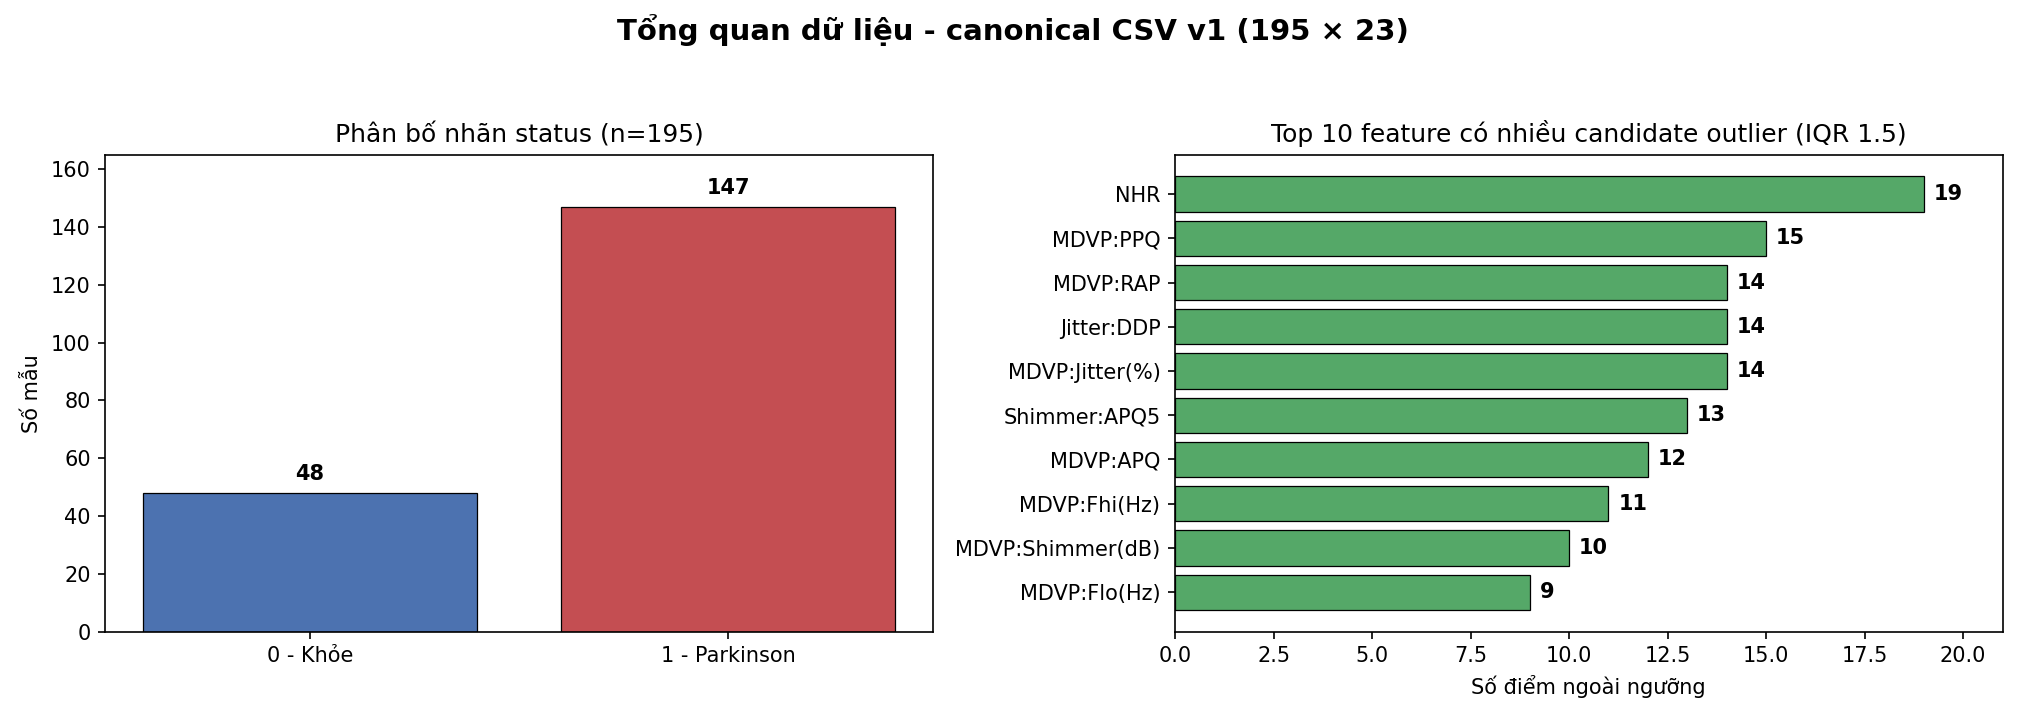
\includegraphics[width=\linewidth]{eda_summary.png}
    \caption{Phân bố nhãn \texttt{status} và các đặc trưng có nhiều candidate outlier theo IQR}
    \label{fig:eda}
\end{figure}
\source{Nhóm tổng hợp từ \texttt{results/quality\_report.md}.}

\subsection{Ngoại lai và độ lệch}

Theo quy tắc IQR hệ số 1,5, 19/22 feature xuất hiện giá trị ngoài ngưỡng; 47/195 mẫu
(24,10\%) chứa ít nhất một candidate outlier. Feature nổi bật là \texttt{NHR} (19 điểm,
9,74\%), \texttt{MDVP:PPQ} (15), các feature jitter \texttt{MDVP:RAP},
\texttt{Jitter:DDP}, \texttt{MDVP:Jitter(\%)} (14 mỗi cột) và \texttt{Shimmer:APQ5} (13).
Ba feature không có candidate outlier là \texttt{MDVP:Fo(Hz)}, \texttt{RPDE} và
\texttt{DFA}. Các điểm ngoại lai chủ yếu là biên độ cao thật của giọng bệnh, nhóm quyết
định giữ nguyên và kiểm soát rò rỉ thay vì loại bỏ mù quáng.

Độ lệch cho thấy 14/22 feature có $|\text{skew}| > 1$, riêng \texttt{NHR} có skew 4,2207
và kurtosis 21,9950, \texttt{MDVP:RAP}/\texttt{Jitter:DDP} skew khoảng 3,36. Đây là dấu
hiệu phân phối lệch mạnh ở nhóm nhiễu và jitter, phù hợp với bản chất của các đại lượng
âm học. Ngoài ra, 26/231 cặp feature có $|r| \ge 0{,}9$; hai cặp gần trùng thông tin là
\texttt{Jitter:DDP} $\approx 3\times$\texttt{MDVP:RAP} và
\texttt{Shimmer:DDA} $\approx 3\times$\texttt{Shimmer:APQ3} với $r = 1{,}0$. Canonical
CSV giữ nguyên các feature này để không thay đổi thông tin dữ liệu gốc.

\section{Tiền xử lý và phân tích thành phần chính}

\subsection{Chuẩn hoá và ma trận đặc trưng}
Nhóm tách $X$ (22 feature) và $y$ (\texttt{status}), sau đó chuẩn hoá z-score bằng
\texttt{StandardScaler}. Ma trận chuẩn hoá $X_s$ có kích thước $195\times22$, trung bình
gần 0 và độ lệch chuẩn gần 1, không có giá trị thiếu. Việc chuẩn hoá trên toàn bộ $X$ chỉ
dùng cho PCA và phân cụm; trong phân loại, bộ chuẩn hoá được đặt trong \texttt{Pipeline} để
fit riêng trên từng fold huấn luyện.

\subsection{Kết quả PCA}

\begin{table}[H]
\centering
\caption{Phương sai giải thích của PCA}
\begin{tabular}{|l|r|}
\hline
\textbf{Thành phần} & \textbf{Tỷ lệ phương sai giải thích} \\
\hline
PC1 & 58,9\% \\
\hline
PC2 & 11,3\% \\
\hline
PC1 + PC2 & 70,2\% \\
\hline
Thành phần đạt ngưỡng $\ge$ 90\% & 6 (tích luỹ 91,61\%) \\
\hline
\end{tabular}
\end{table}

Hai thành phần đầu giữ 70,2\% phương sai; để đạt ngưỡng 90\% phương sai cần 6 thành phần
(tích luỹ 91,61\%). Biểu đồ phân tán PC1-PC2 cho thấy hai nhóm tách một phần nhưng chồng
lấn đáng kể, tức ranh giới bệnh lý không nằm ngay trên hai trục chính.

\begin{figure}[H]
    \centering
    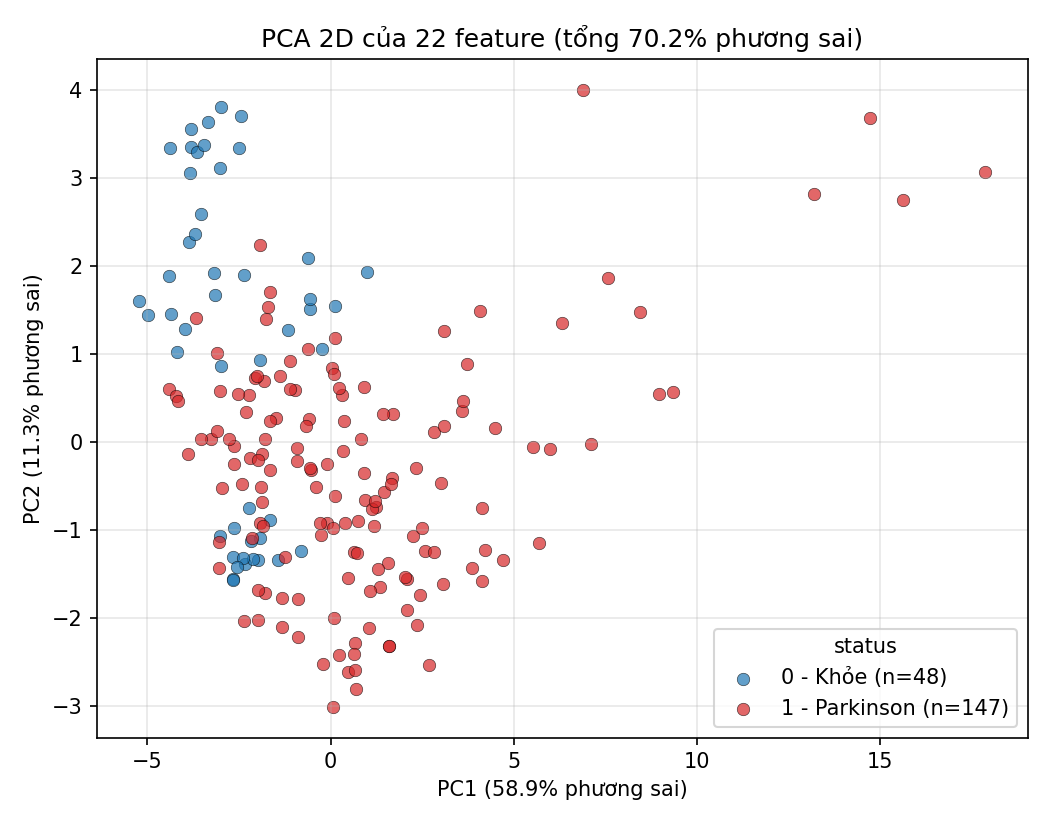
\includegraphics[width=0.78\linewidth]{pca_scatter.png}
    \caption{Scatter PC1-PC2 tô theo \texttt{status}}
    \label{fig:pca_scatter}
\end{figure}
\source{\texttt{results/figures/02\_pca\_scatter.png}.}

\begin{figure}[H]
    \centering
    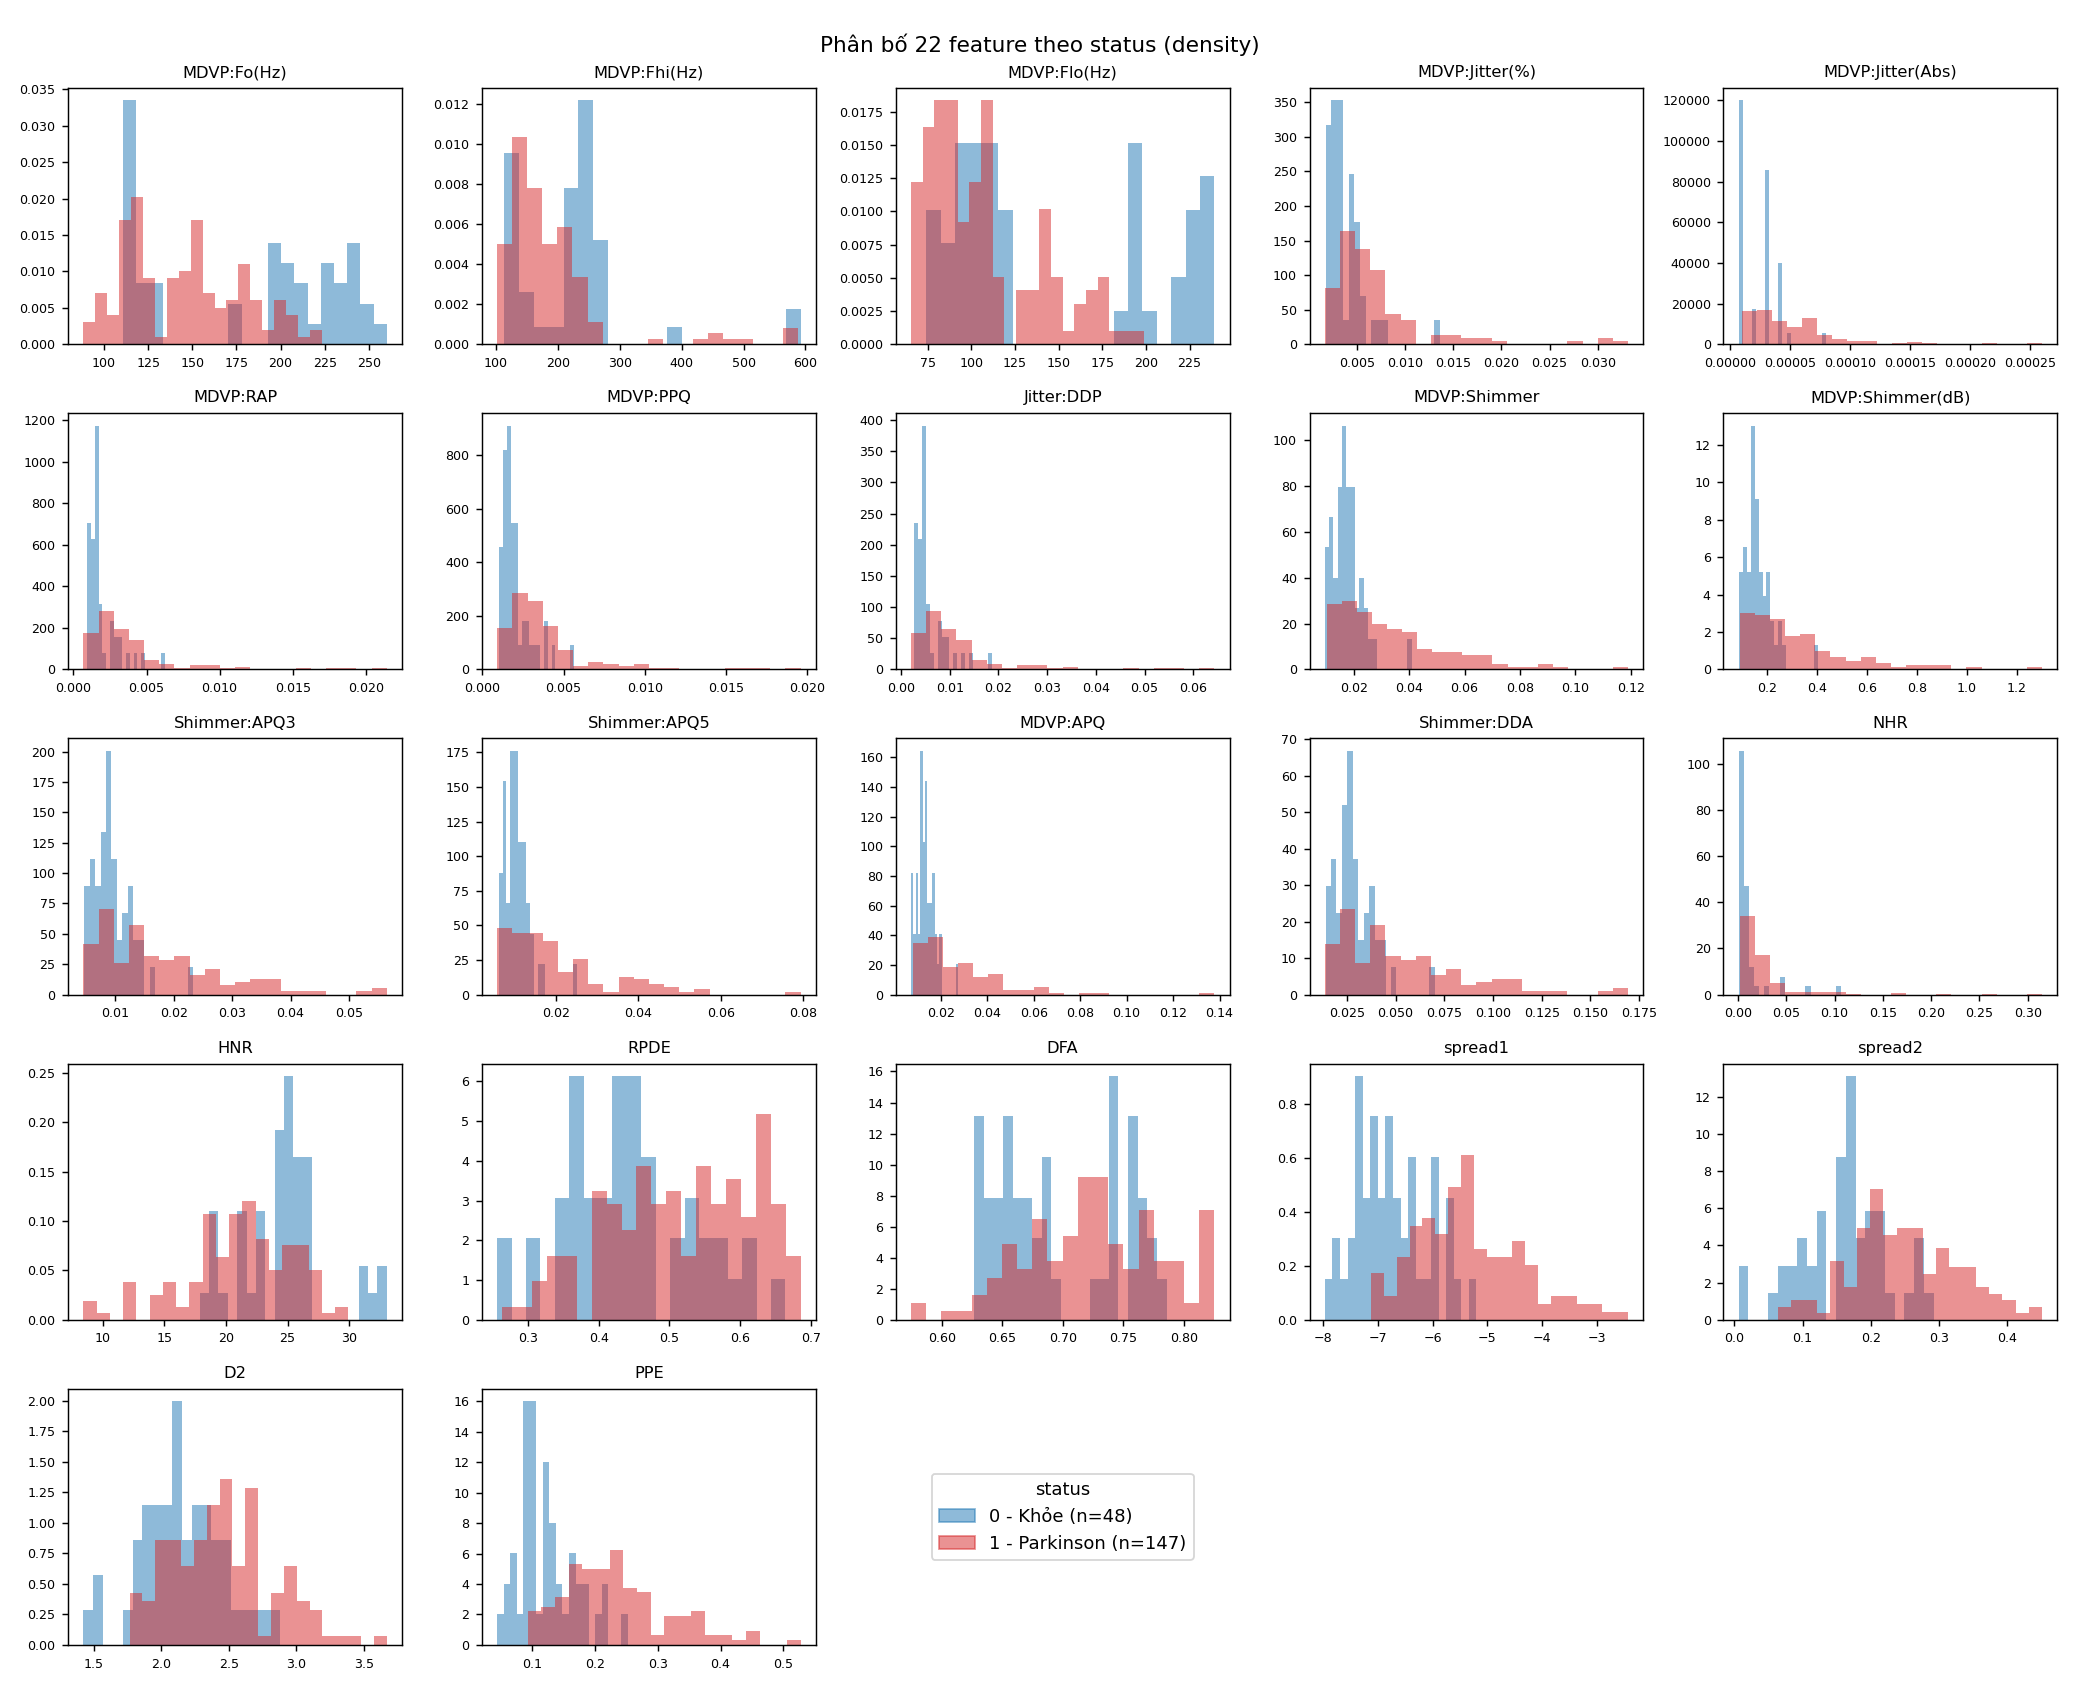
\includegraphics[width=0.84\linewidth]{histograms.png}
    \caption{Histogram 22 feature theo \texttt{status}}
    \label{fig:histograms}
\end{figure}
\source{\texttt{results/figures/m04-t3\_histograms.png}.}

\begin{figure}[H]
    \centering
    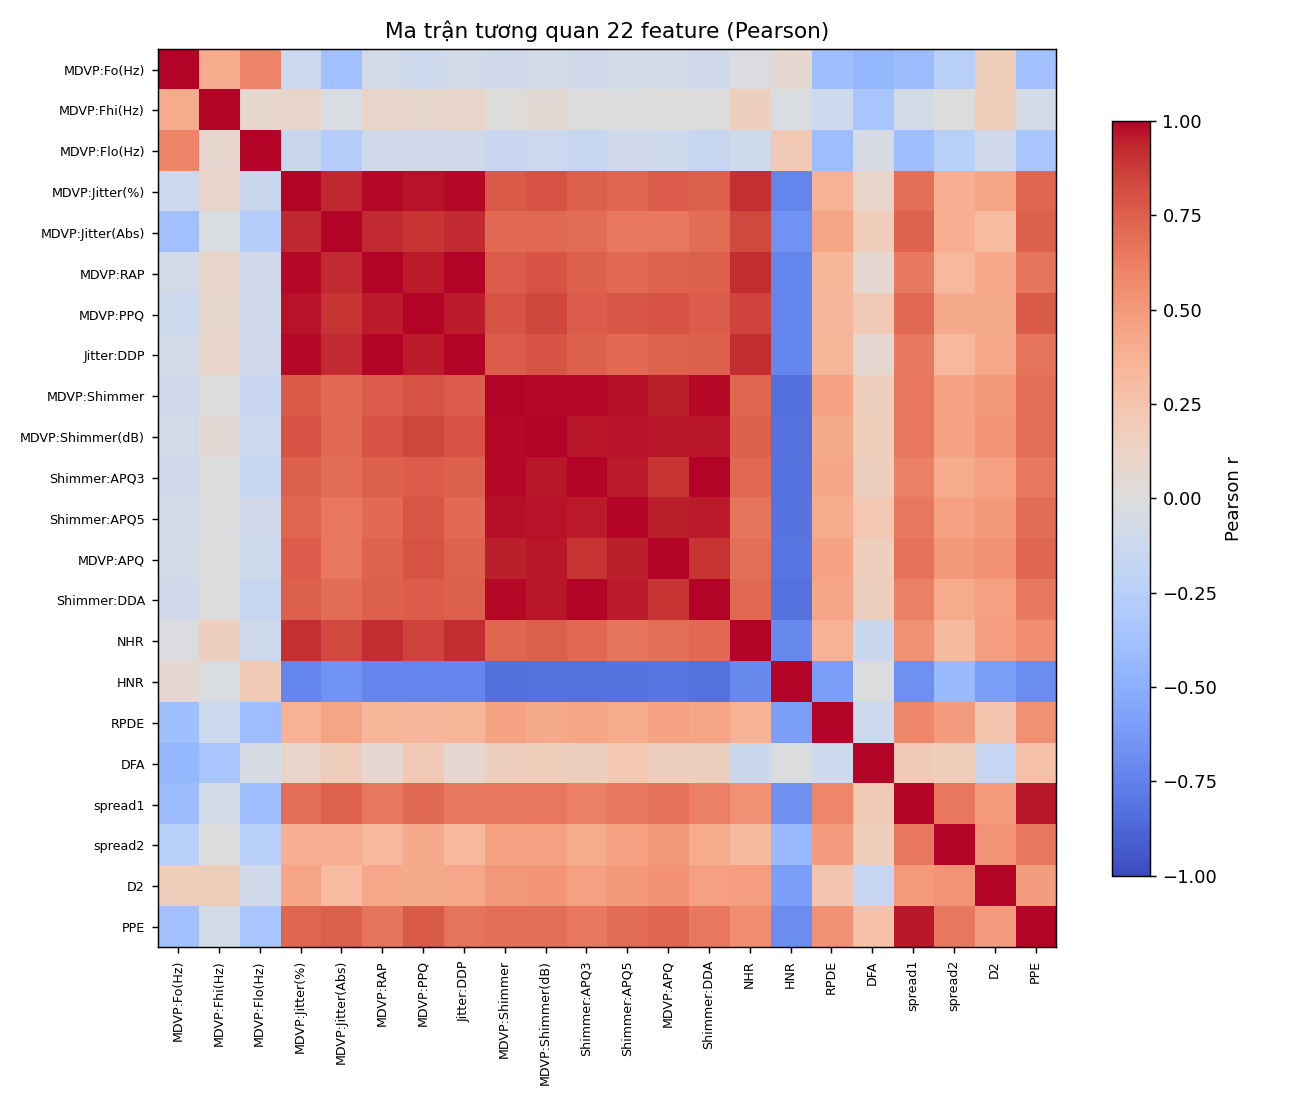
\includegraphics[width=0.84\linewidth]{corr_heatmap.png}
    \caption{Ma trận tương quan Pearson giữa các feature}
    \label{fig:heatmap}
\end{figure}
\source{\texttt{results/figures/m04-t3\_corr\_heatmap.png}.}

Histogram theo nhãn cho thấy nhiều feature có phân phối hai lớp chồng lấn, đặc biệt nhóm
jitter/shimmer; một số feature phi tuyến (RPDE, DFA, PPE) cho phân bố tách biệt hơn. Ma
trận tương quan xác nhận sự lặp thông tin trong nhóm jitter/shimmer như đã mô tả ở mục
trước.

\section{Phân loại có giám sát}

\subsection{Thiết lập thực nghiệm}
Nhóm dùng kiểm định chéo phân tầng 10-fold (seed 42), trong mỗi fold lại chạy tìm lưới 5-fold
trên tập huấn luyện; tiêu chí chọn tham số là F-score macro. Lưới tham số gồm KNN
$n\_neighbors \in \{3,5,7\}$, SVM $C \in \{0{,}1; 1; 10\}$ và Random Forest
$n\_estimators \in \{50; 100\}$. Bộ chuẩn hoá nằm trong \texttt{Pipeline}, fit trên phần
huấn luyện của từng fold.

\subsection{Kết quả}

\begin{table}[H]
\centering
\caption{F-score trên 10-fold CV (mean $\pm$ std)}
\begin{tabular}{|l|c|c|c|}
\hline
\textbf{Mô hình} & \textbf{F-score macro (test)} & \textbf{F-score weighted (test)} & \textbf{F-score macro (train)} \\
\hline
KNN & 0,8757 $\pm$ 0,0742 & 0,9073 $\pm$ 0,0578 & 0,9647 \\
\hline
SVM & \textbf{0,8904 $\pm$ 0,0804} & \textbf{0,9199 $\pm$ 0,0603} & 0,9787 \\
\hline
Random Forest & 0,8737 $\pm$ 0,1171 & 0,9103 $\pm$ 0,0824 & 1,0000 \\
\hline
\end{tabular}
\end{table}

\begin{figure}[H]
    \centering
    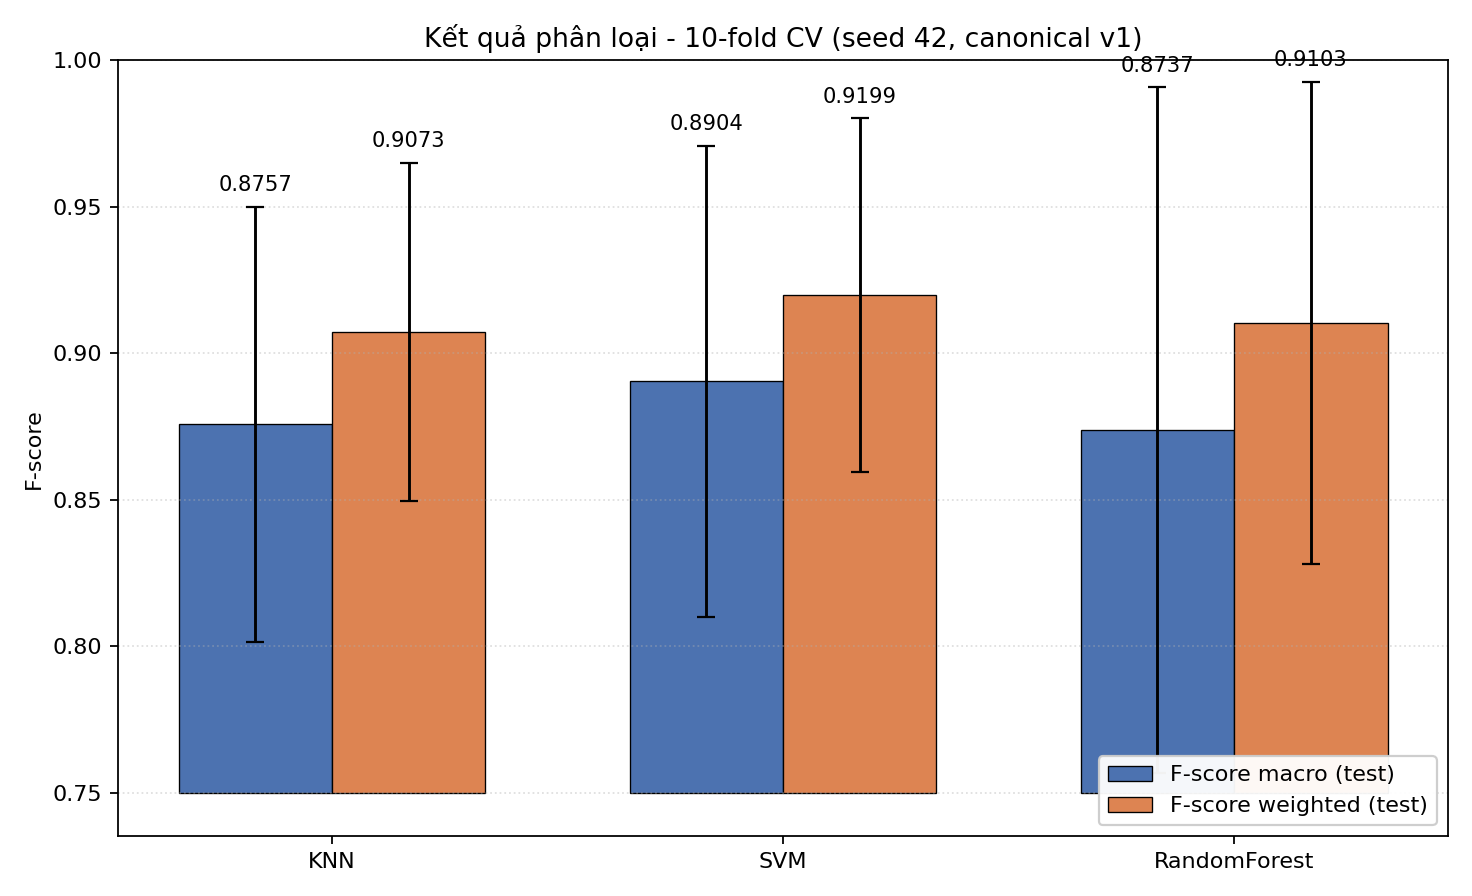
\includegraphics[width=0.86\linewidth]{f1_scores.png}
    \caption{F-score macro và weighted trên 10-fold CV cho ba mô hình}
    \label{fig:f1}
\end{figure}
\source{\texttt{docs/images/f1\_scores.png}.}

Ba mô hình đều đạt F-score macro trên 0,87 trên tập kiểm tra. SVM đạt cao nhất (0,8904),
nhưng chênh lệch giữa các mô hình chỉ khoảng 0,016 - nhỏ hơn độ lệch chuẩn giữa các fold
(0,07-0,12) - do đó báo cáo không kết luận một mô hình tốt nhất một cách chắc chắn.
F-score weighted cao hơn macro ở cả ba mô hình do lớp khỏe (48 mẫu) có tỷ trọng nhỏ.
Random Forest có điểm huấn luyện 1,0000 và độ lệch chuẩn lớn nhất, cho thấy dấu hiệu quá
khớp; KNN và SVM ổn định hơn.

\section{Phân cụm không giám sát và đánh giá ARI}

\subsection{K-Means}
Các mô hình K-Means ($K = 2\dots10$, $n\_init=10$, seed 42) được chạy trên $X_s$; số cụm
được chọn theo silhouette trung bình. Kết quả đầy đủ ở Bảng \ref{tab:kmeans}.

\begin{table}[H]
\centering
\caption{Kết quả K-Means và ARI so với \texttt{status}}
\begin{tabular}{|c|r|r|l|r|}
\hline
\textbf{K} & \textbf{Inertia} & \textbf{Silhouette} & \textbf{Kích thước cụm} & \textbf{ARI} \\
\hline
\textbf{2} & 2817,2 & \textbf{0,4373} & [165, 30] & \textbf{$-$0,0978} \\
\hline
3 & 2076,2 & 0,2763 & [106, 77, 12] & 0,0582 \\
\hline
4 & 1822,4 & 0,2358 & [91, 77, 23, 4] & 0,0583 \\
\hline
5 & 1595,5 & 0,2048 & [73, 64, 32, 22, 4] & 0,1000 \\
\hline
6 & 1442,0 & 0,2138 & [60, 51, 30, 28, 22, 4] & 0,1058 \\
\hline
7 & 1319,8 & 0,2094 & [54, 51, 31, 24, 23, 8, 4] & 0,0882 \\
\hline
8 & 1230,5 & 0,2201 & [53, 35, 32, 23, 23, 15, 10, 4] & 0,0313 \\
\hline
9 & 1157,0 & 0,2265 & [52, 39, 25, 24, 21, 13, 9, 8, 4] & 0,0574 \\
\hline
10 & 1110,7 & 0,1896 & [38, 35, 26, 23, 22, 18, 12, 9, 8, 4] & 0,0481 \\
\hline
\end{tabular}
\label{tab:kmeans}
\end{table}

Silhouette đạt cực đại tại $K = 2$ (0,4373), giảm mạnh ở $K = 3$ (0,2763) và dao động quanh
0,19-0,24 ở các giá trị lớn hơn; đường cong inertia giảm đều, không có điểm gập rõ ràng nên
Elbow chỉ dùng để đối chiếu. Tuy nhiên, ARI tại $K = 2$ là $-0{,}0978$ và trên toàn dải
$K$ chỉ nằm trong $[-0{,}0978; 0{,}1058]$, cho thấy cụm K-Means không khớp ranh giới bệnh
lý. Cụm nhỏ 30 mẫu nằm lệch về phía PC1 dương, nhiều khả năng là nhóm có biên độ cao
thay vì nhóm khỏe mạnh.

\begin{figure}[H]
    \centering
    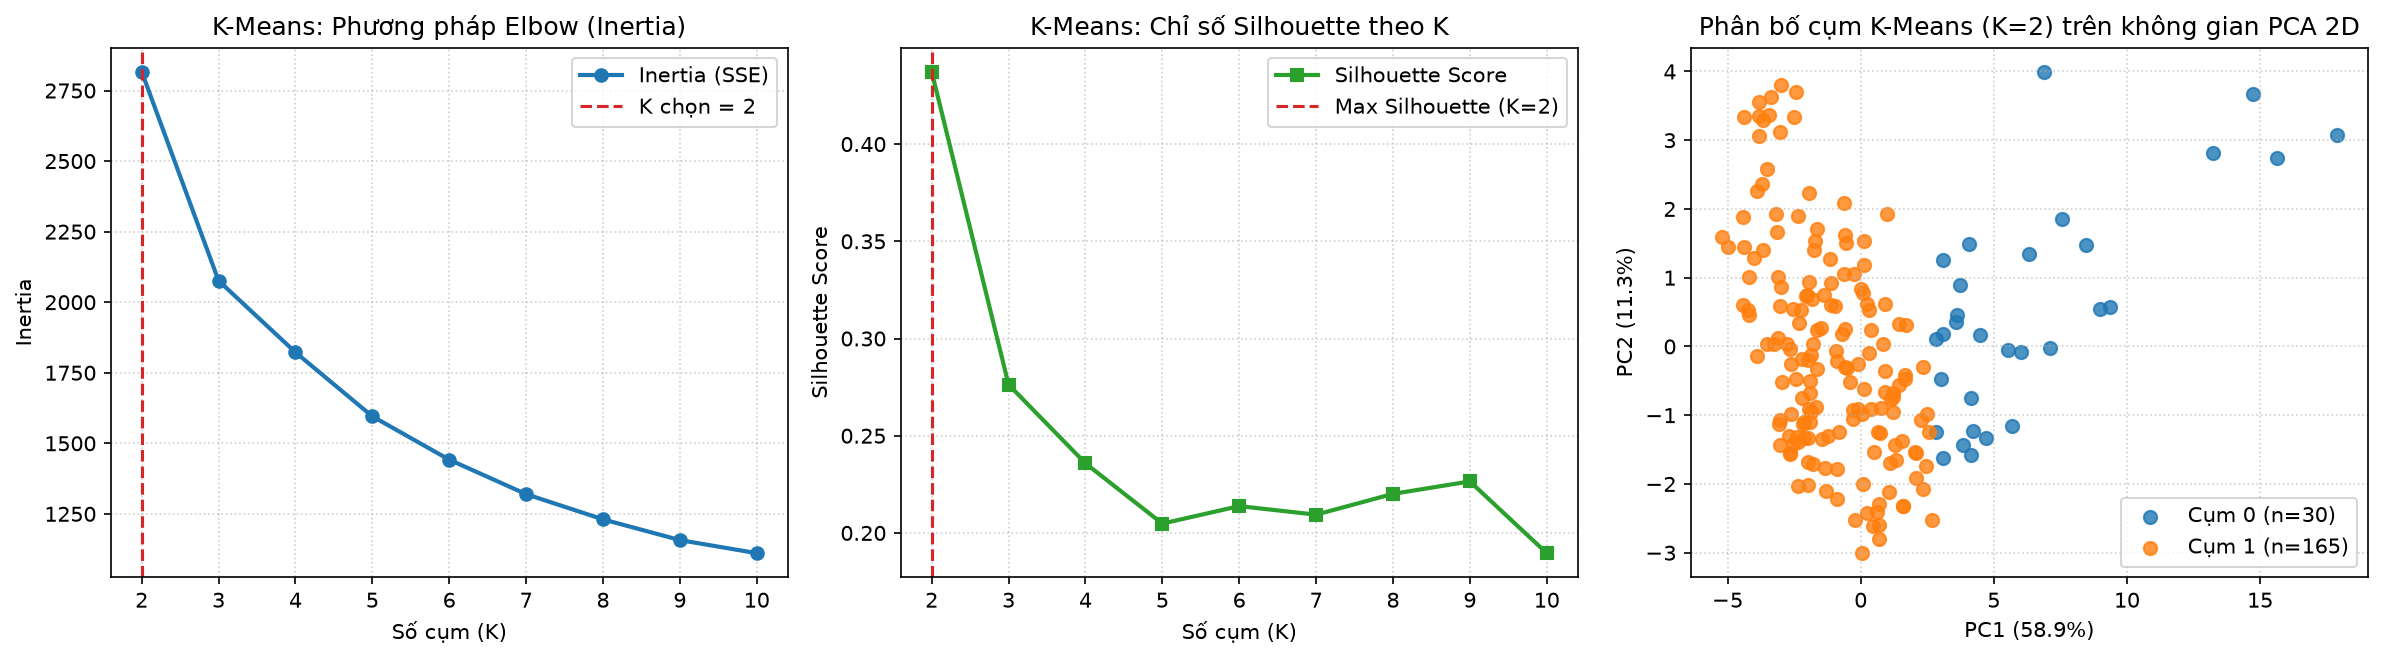
\includegraphics[width=0.92\linewidth]{kmeans_selection.png}
    \caption{Đánh giá K-Means: inertia, silhouette và kích thước cụm theo K}
    \label{fig:kmeans}
\end{figure}
\source{\texttt{results/figures/m06\_kmeans\_selection.png}.}

\subsection{DBSCAN}
Với \texttt{min\_samples = 5}, đường cong k-distance cho điểm uốn tại $\varepsilon = 3{,}37$.
DBSCAN tại cấu hình này tạo \textbf{một} cụm gồm 183 điểm và 12 điểm nhiễu, với ARI
$-0{,}0639$. Khảo sát lưới tham số
($\varepsilon \in \{1{,}5; 2{,}0; 2{,}5; 3{,}0; 3{,}5; 4{,}0; 5{,}0\}$,
\texttt{min\_samples} $\in \{3; 5; 10\}$) cho thấy ARI chỉ nằm trong
$[-0{,}0744; 0{,}1625]$; giá trị cao nhất 0,1625 đạt khi $\varepsilon = 1{,}5$,
\texttt{min\_samples} = 5 nhưng khi đó 149/195 điểm là nhiễu, không có ý nghĩa phân cụm.
Kết quả cho thấy trong không gian 22 chiều chuẩn hoá, mật độ điểm phân bố liên tục và
không hình thành các vùng mật độ tách biệt ứng với hai lớp bệnh/khỏe.

\begin{figure}[H]
    \centering
    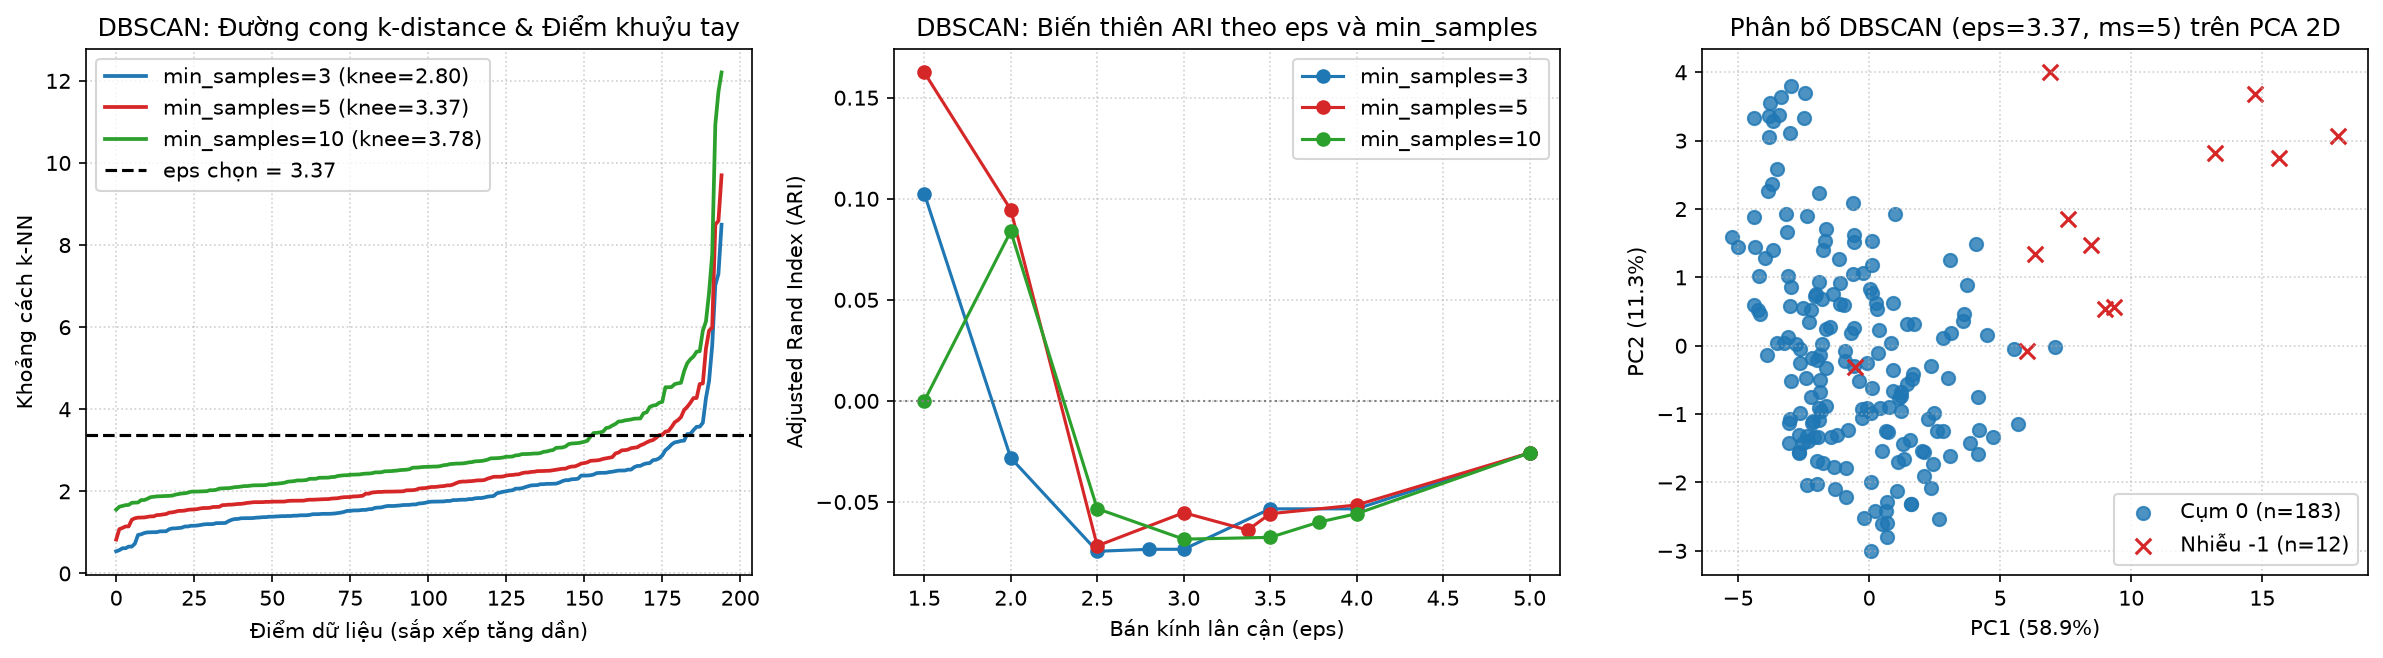
\includegraphics[width=0.92\linewidth]{dbscan_analysis.png}
    \caption{Phân tích DBSCAN: k-distance, cụm/nhiễu và ARI theo tham số}
    \label{fig:dbscan}
\end{figure}
\source{\texttt{results/figures/m06\_dbscan\_analysis.png}.}

\section{Đối chiếu tổng hợp}

\begin{table}[H]
\centering
\caption{Đối chiếu câu hỏi nghiên cứu với kết quả}
\begin{tabular}{|p{1.6cm}|p{6.2cm}|p{6.4cm}|}
\hline
\textbf{Câu hỏi} & \textbf{Kết quả chính} & \textbf{Nhận xét} \\
\hline
RQ1 & 0 NaN/trùng; 19/22 feature có outlier IQR; 47/195 mẫu; nhãn 147/48; 14/22 feature lệch mạnh & Dữ liệu sạch nhưng lệch nhãn/thang đo; cần chuẩn hoá và CV phân tầng \\
\hline
RQ2 & F-score macro 0,8757 (KNN), 0,8904 (SVM), 0,8737 (RF); RF có dấu hiệu quá khớp & Phân loại đạt tốt; chênh lệch giữa mô hình nhỏ so với biến động giữa fold \\
\hline
RQ3 & K-Means K=2 silhouette 0,4373 nhưng ARI $-$0,0978; DBSCAN 1 cụm, 12 nhiễu, ARI $-$0,0639 & Cấu trúc cụm không khớp \texttt{status}; bệnh lý cần mô hình có giám sát \\
\hline
\end{tabular}
\end{table}

Kết quả cho thấy quy trình khai phá dữ liệu vận hành nhất quán: dữ liệu đầu vào duy nhất,
mọi bước tái lập với seed 42, và các kết luận được giới hạn đúng theo độ biến động của số
liệu. Phân loại có giám sát giữ vai trò chính trong bài toán, trong khi phân cụm phục vụ
đối chiếu và nhận định giới hạn của tín hiệu không gian đặc trưng.
